% astr5400/hw2/hw2.tex
%
% Omkar H. Ramachandran
% omkar.ramachandran@colorado.edu
%
% LaTeX writeup of HW2
%

\documentclass[english]{article}
\usepackage[T1]{fontenc}
\usepackage[latin9]{inputenc}
\usepackage{geometry}
\geometry{verbose,tmargin=1.5in,bmargin=1.5in,lmargin=1.5in,rmargin=1.5in}
\usepackage{babel}
\newcommand{\GeV}{\,{\rm GeV}}
\usepackage{graphicx}
\graphicspath{{./plots/}}
\usepackage{hyperref}
\usepackage{listings}
\usepackage{color}

\lstdefinestyle{custompy}{
  belowcaptionskip=1\baselineskip,
  breaklines=true,
  frame=L,
  xleftmargin=\parindent,
  language=Python,
  showstringspaces=false,
  basicstyle=\footnotesize\ttfamily,
  keywordstyle=\bfseries\color{green},
  commentstyle=\itshape\color{red},
  identifierstyle=\color{black},
  stringstyle=\color{blue},
}


\lstset{escapechar=@,style=custompy}

\begin{document}
\title{ASTR 5400 : Homework 3}
\author{Omkar H. Ramachandran}

\maketitle

\section{Why is a potential flow a good approach to solve the system?}
Solving a system by means of a potential flow, involves writing the velocity
flow as the gradient of a scalar potential. 
For this condition to be true, we require the fluid to be incompressible.
Since the problem assumes that the fluid is irrotational, writing the velocity
function as the gradient of a potential is acceptable.
\begin{figure}
	\centering
	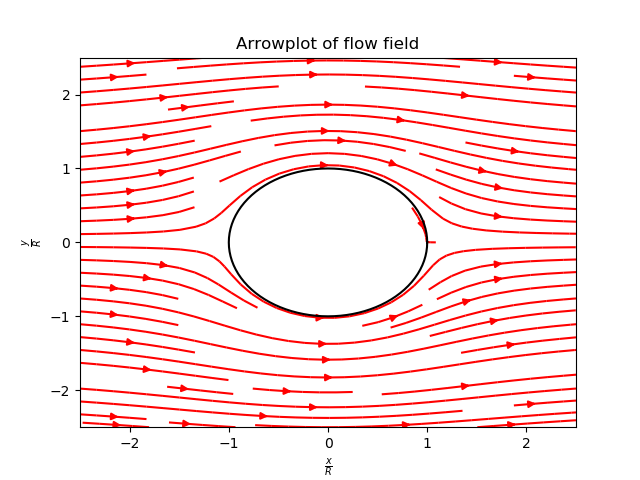
\includegraphics[width=0.75\textwidth]{arrowplotp2.png}
	\caption{Arrowplot of flow function found in Problem 2}
	\label{fig:streamplot1}
\end{figure}

\section{Find the velocity potential}
Note: I was slightly confused as to what the question was asking. Did you
want us to solve Laplace's equation in Polar coordinates or do you just want
us to plug in the given velocity function and show that it satisfies the ODE? 
(Given that I'm presently drowning in a wave of nostalgia from Quantum 1,
I'm going to solve the whole thing)

Laplace's equation in $(r,\theta)$ looks as follows:
$$ \nabla^{2} \phi = \frac{1}{r}\frac{\partial}{\partial r}\left(
	r\frac{\partial \phi}{\partial r}\right) + 
	\frac{1}{r^{2}}\frac{\partial^{2} u}{\partial\theta^{2}}
$$
From the 20 different times we did this Quantum I, the obvious way forward is
to assume that $\phi=R(r)\Theta(\theta)$ and following up with a good plug and 
chug (To keep the notation clean $P^{(ni)}$ refers to 
$\frac{\partial^{n} P}{\partial i^{n}}$):
$$ \frac{1}{r}(rR^{(r)})^{(r)}\Theta + \frac{1}{r^{2}}R\Theta^{(2\theta)}=0$$
Rearranging,
$$ \frac{r^{2}R^{(2r)}+rR^{(r)}}{R} = -\frac{\Theta^{(2\theta)}}{\Theta}$$
The only way this condition can be true is if both sides of the equation
independently equal to a constant.
Therefore - with foresight from Quantum 1 -, we set this constant to 
$-\lambda=-n^{2}$, to get
$$ \frac{\Theta^{(2\theta)}}{\Theta} = n^{2}$$
Since this is just the Helmholtz equation, we know that the solution is simply
$$ \Theta = a_n\cos(n\theta)+b_n\sin(n\theta) \;\;\;\;\; n\in\mathbf{N}$$
We can get rid of one of the two trig functions by setting our coordinate
system properly (i.e, if the flow is purely along $\hat{x}$, then 
$U(a,\theta)[x]=0$ iff $\theta=\pm\pi/2$). 
Thus, our rectified equation is simply
$$ \Theta = a_n\cos(n\theta)\;\;\;\;\; n\in\mathbf{N}$$
The $R$ equation is as follows:
$$ r^{2} R^{(2r)}+rR^{(r)}+n^{2}R=0 $$
This is formally known as a Cauchy-Euler equation and it's solution is a little 
less obvious - you can't do the standard 'plug in $\exp(-r)$' because the equation
is not constant coefficient. 
From the accumulated wisdom of solving Schrodinger's equation in 
a spherically symmetric potential, I'm going to guess that the solution looks
as follows:
$$ R(r) = c_{1}r^{n}+c_{2}r^{-n} $$
Normally, we would throw away the $r^{n}$ solution, but remember that we are
solving for the potential - which \textit{can} go to $\infty$ as $r$ increases.
Therefore, our unseperated equation is the following:
$$\phi(r,\theta)=a_n(c_{1}r^{n}+c_{2}r^{-n})\cos(\theta)$$
Now, we know that as $r\rightarrow \infty$, $\nabla\phi\rightarrow U \ \forall \theta$. 
Thus, $n$ is obviously 1.
Any other function would blow up at $\infty$.
$$ \lim_{r\rightarrow\infty}\nabla\phi = 
	\lim_{r\rightarrow\infty}((a_nc_{1}-\frac{a_nc_{2}}{r^{2}})\cos(\theta),
	-\frac{1}{r}a_n(c_1r+c_2/r)\sin(\theta))
$$
Getting rid of terms that vanish, we are left with
$$ \lim_{r\rightarrow\infty}\nabla\phi = 
	a_nc_{1}(\cos\theta,-\sin\theta)
$$
The $(\cos\theta,-\sin\theta)$ simply orients the velocity vector in the right
direction.
Since the magnitude is $U$ at large distances, we have
$$ a_nc_{1} = U$$
Similarly, we know that for $r=a$ and $\theta=0$,$\nabla\phi[y]=0$ - on the top
side of the cylinder at $r=a$, the flow is purely along $x$.
Thus,
$$ \nabla\phi = ((U-\frac{a_nc_{2}}{r^{2}})\cos(\theta),
	-\frac{1}{r}(Ur+a_nc_{2}/r)\sin(\theta))
$$
The second term is zero. 
Thus, we are left with
$$ U = a_nc_{2}a^{-2} \rightarrow a_nc_{2} = Ua^{2} $$
And we're done! Putting all of this together, we come up with the required
potential function:
$$ \phi = U\left(r+\frac{a^{2}}{r}\right)\cos(\theta)$$
That was fun! The plot of this stream function looks as follow. 
The streamplot of the solution is as in Figure \ref{fig:streamplot1}
\begin{figure}
	\centering
	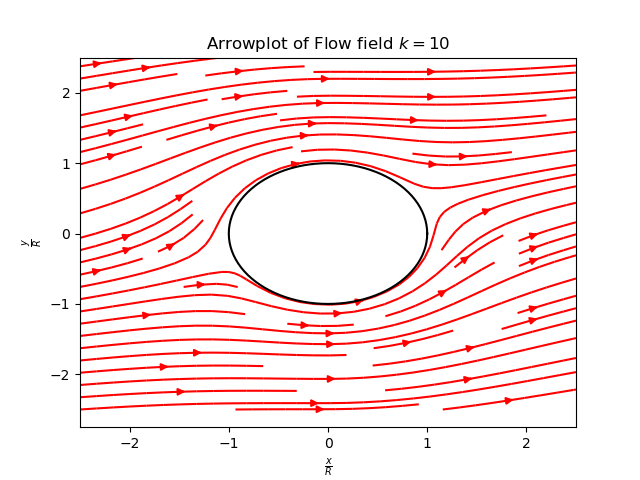
\includegraphics[width=0.75\textwidth]{arrowplotp3.png}
	\caption{Streamplot of the given flow field for $k=10$. 
	Comparing with \ref{fig:streamplot1} highlights the main difference: the
	rotation of the cylinder causes the system to become spherically asymmteric,
	specifically by slowing down the fluid flowing on the side of the cylinder
	where the local rotation vector is counter to the natural velocity of the fluid}
	\label{fig:streamplot2}
\end{figure}

\section{The cylinder rotates!}
If the velocity potential is changed to include rotation, 
$$  \phi = U\left(r+\frac{a^{2}}{r}\right)\cos(\theta) + \frac{k\theta}{2\pi}$$
Then, our velocity field looks as follows:
$$ \nabla\phi = ((U-\frac{Ua^{2}}{r^{2}})\cos(\theta),
	-\frac{1}{r}((Ur+Ua^{2}/r)\sin(\theta)+\frac{k}{2\pi}))
$$
The streamplot of this field is as shown in Figure \ref{fig:streamplot2}.
The main difference between this plot and Figure \ref{fig:streamplot1} lies
in the fact that the spherical symmetry is broken with the new potential.
In specific, the fluid flowing on the side of the cylinder where the local
velocity vector is exactly opposite to the fluid velocity vector slows down,
while the other side speeds up.

\section{Apply Bernoulli's Principle}
From Bernoulli's Principle, we know that in the absence of external body forces,
we have the following:
$$ \intop dl.\left[\nabla\left[\frac{1}{2}u^{2}\right]+\frac{\nabla P}{\rho}\right] =0$$
Since we know that the fluid is incompressible,
$$ \intop dl.\nabla\left[\left[\frac{1}{2}u^{2}\right]+\frac{P}{\rho}\right] = 0$$
Now, we can use the gradient theorem to assert that
$$ \intop_{[p,q]} dl.\nabla\Phi = \Phi(q)-\Phi(p)$$
Choosing to do the integral from $\theta=-\pi/2$ to $\theta=\pi/2$ (i.e, from 
$(-R,0)$ to $(R,0)$), we have
$$  \intop dl.\nabla\left[\left[\frac{1}{2}u^{2}\right]+\frac{P}{\rho}\right] = 
	\left[\frac{1}{2}u(\theta=0)^{2}\right]-\left[\frac{1}{2}u(\theta=\pi)^{2}\right]
	-\frac{\Delta P}{\rho}=0
$$
Since $u=\nabla \phi$, we have $u(\theta=0) = (0,U/a-k/2\pi a)$ and $u(\theta=\pi/2) = (0,-U/a-k/2\pi a)$.
The pressure difference is negative because the gradient theorem gives us $P(q)-P(p)$ 
Evaluating the quadratic, difference, only the $2ab$ term survives, to give us
$$ \frac{2Uk}{\pi a^{2}} = \frac{|\Delta P|}{\rho}$$
Thus,
$$ |P| = \rho\left(\frac{2Uk}{\pi a^{2}}\right) $$
Now, the velocity difference is purely in the $\hat{y}$ direction, since the
$x$ velocities at the two end points are identical.
Thus, the pressure has to be along $\hat{y}$. Therefore,
$$ P = \frac{2\rho Uk}{\pi a^{2}}\hat{y}$$
The force is just the pressure per unit area, thus,
$$ F = 2\rho Uk \hat{y}$$
\section{What kinds of speeds are needed to generate lift?}
To achieve lift, the $F$ calculated in the previous section has to balance
gravity. Thus,
$$ g = 2\rho Uk$$
We are given that $U=100\ m/s$ and $\rho = 1.2\ kg/m^{3}$ (at Sea level)
Thus,
$$ k = \frac{g}{2U\rho} = \frac{10}{240} = 4.1\times 10^{-2}\ s^{-1}$$
This corresponds to roughly four revolutions per minute and a half.
The energy corresponding to this rotation is
$$ E = \frac{1}{4}Mr^{2}\omega^{2}$$
So, it really depends on $r$. If the rod is $10\ m$ long, for instance,
$$ E = \frac{1}{4}1.6\times10^{4} J$$
Which is still well within the performance capabilities of an aircraft
- or even a engine.
One horsepower is about $750\ J$ and a typical car has a couple hundred.

\section{Examples of the Magnus effect}
There are lots of really cool examples of the Magnus effect. 
In sport, two examples leap to mind: 
\begin{itemize}
	\item The drift of a table-tennis - or ping ping - ball is almost entirely 
		based on the Magnus effect. Understanding how the ball moves and adjusting
		one's next shot is critical to winning a game of table-tennis. And given
		that the surface isn't rough enough for spin to be effective, the magnus
		drift of the ball is the dominant effect
	\item The dip and drift of a spinning cricket ball also depend on the Magnus
		effect. Interestingly, the swing of a cricket ball depends on the fact
		that one side of the ball is rougher than the other and not on the Magnus
		effect[1]. Dipping the ball is a bit of an advanced move in 
		cricket. In the 12ish years that I played the sport, I can count the number
		of spin bowlers who could effectively dip the ball - when they do, however,
		they are a veritable nightmare to play.
\end{itemize}

There was a cool idea that the Germans tried in the 1920s, where they tried
getting a ship to sail using a central rotating rot in place of traditional
sails. 
Sadly though, the rod couldn't generate enough force to be used effectively.
The thrust generated was lower than that of a traditional motor of the same
overall power output.[2]

The magnus effect has been used to replace the traditional wingfoil of an 
aircraft[3]. Given that most aircraft in the modern
age use wingfoils and not a giant moving rod, it wasn't particularly
effective.

\section*{References}
\begin{itemize}
	\item https://en.wikipedia.org/wiki/Magnus\_effect\#In\_sports 
	\item https://www.grc.nasa.gov/WWW/K-12/airplane/cyl.html
	\item https://books.google.com/books?id=xSgDAAAAMBAJ
\end{itemize}

\end{document}
